\documentclass[portuguese]{sbc2025}%
 
%\usepackage{graphicx}% já está incluido na classe
%\usepackage[utf8]{inputenc} % obsoleto, desnecessário

\usepackage[misc,geometry]{ifsym} 
 
%%%%  %\usepackage{fontspec}

%% Os problemas com a classe eram originados por carregarem ambos os
%% pacotes fontenc e fontspec simultaneamente. Agora a classe detecta
%% qual engine está em uso e se for o pdflates então carrega o
%% fontenc. Se forem o xelatex ou lualatex então carrega o
%% fontspec. Eu particularemnte prefiro o lualatex ou o xetex


% \usepackage{fontawesome} %%% incluido na classe. Desnecessário
% chamá-lo aqui


%%%% \usepackage{academicons}
%%%% outro encrenqueiro que se tornou desnecessario. Deste typeface só
%%%% se usava o glifo do orcid e o codigo interno bombava.
%%%% Substitui pelo pacote orcidlink (carregado internamete na classe)
%%%% e consertei o codigo na classe.


%\usepackage{color} % carregada dentro da classe
%\usepackage{hyperref} % carregada dentro da classe

\usepackage{aas_macros}
\usepackage[bottom]{footmisc}

%\usepackage{supertabular}
%\usepackage{multicol}
%\usepackage{multirow}
%% O pacote tabularray é muito melhor para
% a criacao de tabela complexas e/ou loooongas; tudo de modo simples.
%% Torna o uso de multicol e multirow desnecessarios

\usepackage{tabularray}


\usepackage{afterpage}
\usepackage{url}
\usepackage{pifont}
\usepackage{lipsum}

\setcitestyle{square}


\definecolor{engtitle}{rgb}{0.5,0.5,0.5}
\definecolor{orcidlogo}{rgb}{0.37,0.48,0.13}
\definecolor{unilogo}{rgb}{0.16, 0.26, 0.58}
\definecolor{maillogo}{rgb}{0.58, 0.16, 0.26}
\definecolor{darkblue}{rgb}{0.0,0.0,0.0}
\hypersetup{colorlinks,breaklinks,
            linkcolor=darkblue,urlcolor=darkblue,
            anchorcolor=darkblue,citecolor=darkblue}
%\hypersetup{colorlinks,citecolor=blue,linkcolor=blue,urlcolor=blue}

%%%%%%% IMPORTANT: We disable hyperlinks by default with this line, to avoid the error "\pdfendlink ended up in different nesting level" while writing.
%\hypersetup{draft}

\jid{UESPI-PRP-CCOMP}
\jtitle{Trabalhos de Conclusão de Curso do Bacharelado em Ciência da Computação, 202X, XX:1}
% \issn{1519-8219}
% \doi{10.5753/reic.202X.XXXXXX}
\copyrightstatement{This work is licensed under a Creative Commons Attribution 4.0 International License}
\jyear{202X}

\category{Artigo de Pesquisa}
% \category{Artigo de Desenvolvimento Tecnológico}
% \category{Artigo de Startup}
\title[Artigo de TCC da CCOMP UESPI-Piripiri 2025]{Artigo de TCC da Ciência da Computação da Universidade Estadual do Piauí de Piripiri}
\engtitle{\textcolor{engtitle}{UESPI-Piripiri's CS final work paper}}

%THE ORCID IS MANDATORY FOR EACH AUTHOR IN JBCS

\author[Santos et al. 202X]{
\affil{\textbf{Primeiro Autor}~\orcidlink{0000-0000-0000-0000}~~[{Universidade Estadual do Piauí}~|\href{mailto:primeiro@aluno.uespi.br}{{\textit{primeiro@aluno.uespi.br}}}~]}

\affil{\textbf{Segundo Autor}~\orcidlink{0000-0000-0000-0000}~~[{Universidade Estadual do Piauí}~|\href{mailto:segundo@aluno.uespi.br}{{\textit{segundo@aluno.uespi.br}}}~]}

\affil{\textbf{Terceiro Autor}~\orcidlink{0000-0000-0000-0000}~~[{Universidade Estadual do Piauí}~|\href{mailto:terceiro@aluno.uespi.br}{{\textit{terceiro@aluno.uespi.br}}}~]}

\affil{\textbf{Alcemir Rodrigues Santos}~\orcidlink{0000-0001-8880-2996}~\textcolor{blue}{\faEnvelopeO}~~[{Laboratório de Engenharia de Software | Universidade Estadual do Piauí}~|\href{mailto:alcemir@prp.uespi.br}{~{\textit{alcemir@prp.uespi.br}}}~]}

}

\begin{document}

\begin{frontmatter}

\maketitle

\begin{mail}
Universidade Estadual do Piauí, Av. Pres. Castelo Branco, 180 - Petecas, Piripiri - PI, 64260-000, Brasil. 
\end{mail}


\begin{abstract-pt}
    Este texto, em formato de artigo científico, tem por objetivo apresentar o novo modelo para TCC do Bacharelado em Ciência da Computação do Campus de Piripiri da Universidade Estadual do Piauí, descrevendo suas principais características e explicando como deve ser utilizado. Esta versão, mais especificamente, deve ser utilizada exclusivamente para artigos escritos em português. O resumo em português, como pode-se notar neste exemplo, deve vir antes do resumo em inglês (abstract) e ter entre 500 e 750 palavras.
\end{abstract-pt}

\begin{abstract-en}
    This text, formatted as a scientific article, aims to present the new UESPI Piripiri TCC paper template, describing its main features and explaining how it should be used. This version, more specifically, should be used exclusively for articles written in Portuguese. The abstract in Portuguese, as you can see in this example, must be before the abstract in English and must have between 500 and 750 words.
\end{abstract-en}

\begin{pchaves}
Anais de evento, Modelo, SBC OpenLib, Indexação
\end{pchaves}

\begin{keywords}
Proceedings, Template, SBC OpenLib, Indexing
\end{keywords}

\begin{dates}
% This information will be provided by the editor before publishing the paper
\noindent{\sffamily\textbf{Recebido/Received:}} DD Month YYYY~~~$\bullet$~~~
{\sffamily\textbf{Aceito/Accepted:}} DD Month YYYY~~~$\bullet$~~~
{\sffamily\textbf{Publicado/Published:}} DD Month YYYY
\end{dates}


%\begin{license}
%Published under the Creative Commons Attribution 4.0 International Public License (CC BY 4.0)
%\end{license}

\end{frontmatter}

% ============

 \section{Introdução}
\label{sec:intro}

A \textbf{introdução} do seu artigo deve apresentar as partes do seu artigo. De maneira geral, o ideal é que o leitor consiga entender \textit{(i)} o contexto, \textit{(ii)} o problema, \textit{(iii)} a literatura existente atacando aquele problema, \textit{(iv)} o método que você utilizou para enfrentar o problema, \textit{(v)} os resultados alcançados e \textit{(vi)} suas contribuições e \textit{(vii)} conclusões (ou considerações finais). Ela pode ser entendida como uma expansão do resumo do artigo. É comum ainda, que autores decidam por apresentar o restante do documento no decorrer do texto ou no seu último paragrafo como faremos a seguir.

O restante do documento é organizado como segue. {\color{blue} Todo texto \textbf{azul} que você encontrar em seguida é aleatório. Ele foi utilizado somente para preencher o documento.}
A Seção \ref{sec:fundamentacao} apresenta a fundamentação teórica. 
A Seção \ref{sec:metodologia} apresenta a metodologia
A Seção \ref{sec:resultados} apresenta os resultados (esperados no caso de projeto de pesquisa). 
Por fim, a Seção \ref{sec:conclusao} apresenta a conclusão do artigo.
 \section{Fundamentação Teórica}
\label{sec:fundamentacao}


\subsection{Observações sobre a compilação do documento}

A classe \textsl{sbc2025} é projetada para trabalhar com os \textit{engines} pdftex e luatex. Dessa forma, deve-se compilar o documento 
\begin{enumerate}
    \item no Overleaf, ajustando no menu opção de compilação para \textbf{xelatex} ou \textbf{lualatex}.\footnote{Os engines são denominados xetex e luatex. Já os comandos de compilação são \textsl{xelatex} e \textsl{lualatex}.}
    \item se compilando localmente, na sua IDE faça o ajuste do compilador. Se usuário raiz, no terminal de comando, digite \textsl{xelatex filename} ou \textsl{lualatex filename}. Não é necessário digitar a extensão \textsl{tex}.
\end{enumerate}

A classe \textsl{sbc2025} inclui internamente os seguintes pacotes:     \texttt{xcolor}; \texttt{graphicx}; \texttt{amsmath} \texttt{amssymb}; \texttt{hyperref};     \texttt{babel}.

\noindent consequentemente, não há necessidade de incluí-los no preâmbulo.

{\bfseries Quem tentar compilar usando a opção \texttt{pdflatex} no Overleaf vai receber uma mensagem de erro solicitando o usuário a ajustar a opção de compilação.}

Para a pergunta \textit{Por que não funciona com o \texttt{pdflatex}}?  A resposta é: \textbf{fontes!} Pdflatex usa um esquema de codificação de fontes complexo. 
O fonte \texttt{academicons}\footnote{Do fonte em questão usa-se apenas o glifo associado ao OrchID.} não tem as definições necessárias para uso com o \texttt{pdflatex}. Enquanto isso não for realizado, \texttt{pdflatex} não pode ser usado. 



\subsection{Outra subseção}

Evite deixar \textbf{uma única} subseção dentro de uma seção. Nestes casos, é possível utilizar-se de conectores para remover a divisão da subseção e escrever o texto da seção de forma direta. Não levantando assim, a expectativa de uma segunda subseção.

 \section{Metodologia}
\label{sec:metodologia}



\subsection{Exemplos de istas}

\begin{itemize}
\item Esse é um exemplo de lista de tópicos. 
{\color{blue}
\item Lorem ipsum dolor sit amet, consectetur adipiscing elit, sed do eiusmod tempor incididunt.
\item Lorem ipsum dolor sit amet, consectetur adipiscing elit, sed do eiusmod tempor incididunt ut labore et dolore magna aliqua. Ut enim ad minim veniam.
\item Lorem ipsum dolor sit amet, consectetur adipiscing elit, sed do eiusmod tempor incididunt ut labore et dolore magna aliqua. Ut enim ad minim veniam.}
\end{itemize}


\begin{enumerate}%
\item Esse é um exemplo de lista numerada.
{\color{blue}
\item Lorem ipsum dolor sit amet, consectetur adipiscing elit, sed do eiusmod tempor incididunt.
\item Lorem ipsum dolor sit amet, consectetur adipiscing elit, sed do eiusmod tempor incididunt ut labore et dolore magna aliqua. Ut enim ad minim veniam.
\item Lorem ipsum dolor sit amet, consectetur adipiscing elit, sed do eiusmod tempor incididunt ut labore et dolore magna aliqua. Ut enim ad minim veniam.}
\end{enumerate}



\subsection{Exemplos de inclusão de imagens}

Referência de figuras no texto \textbf{Figure \ref{Fig1}} que se expandem em uma única coluna.\textbf{Figure \ref{Fig1}}.


\begin{figure}
\begin{center}
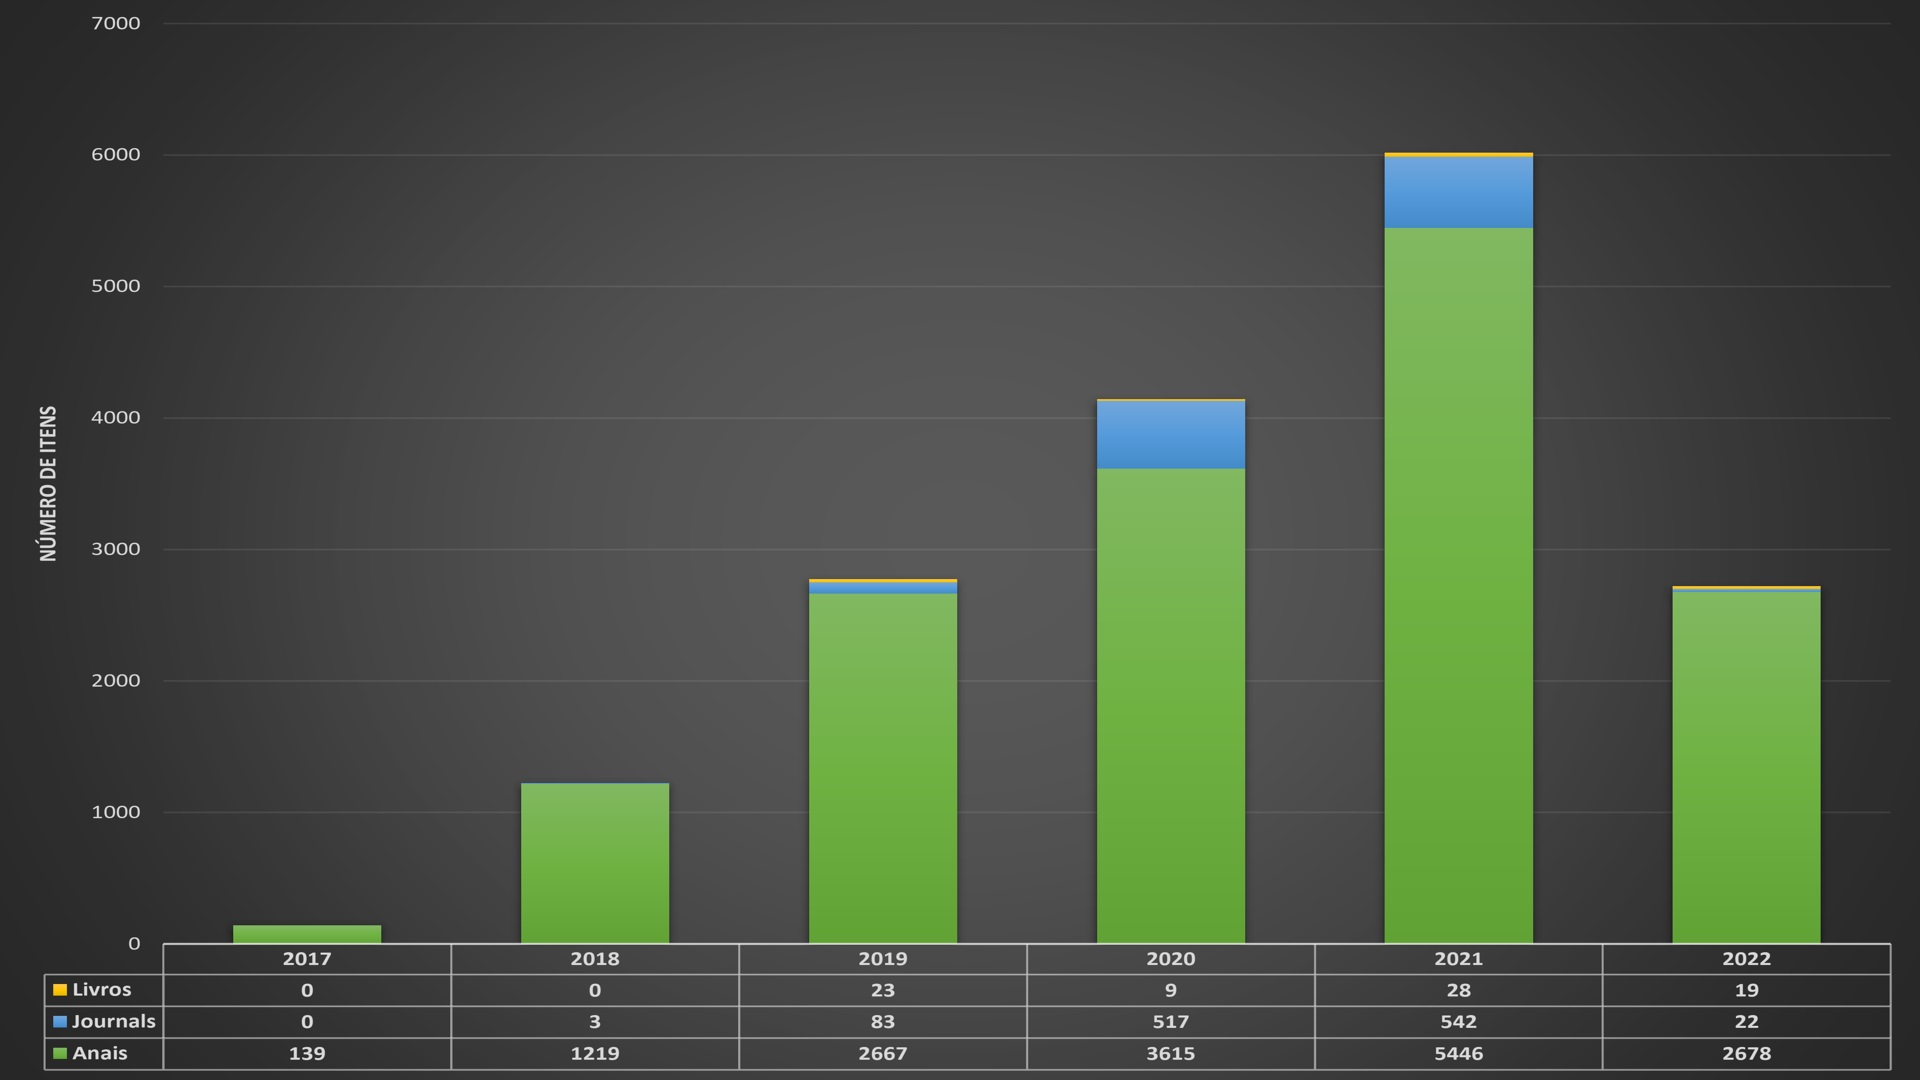
\includegraphics[width=\columnwidth]{imagens/sol.jpg}
\caption{Exemplo de legenda de figura.}\label{Fig1}
\end{center}
\end{figure}

Referência de figuras no texto \textbf{Figure \ref{Fig2}} que se expandem pelas duas colunas.

\begin{figure*}
\begin{center}
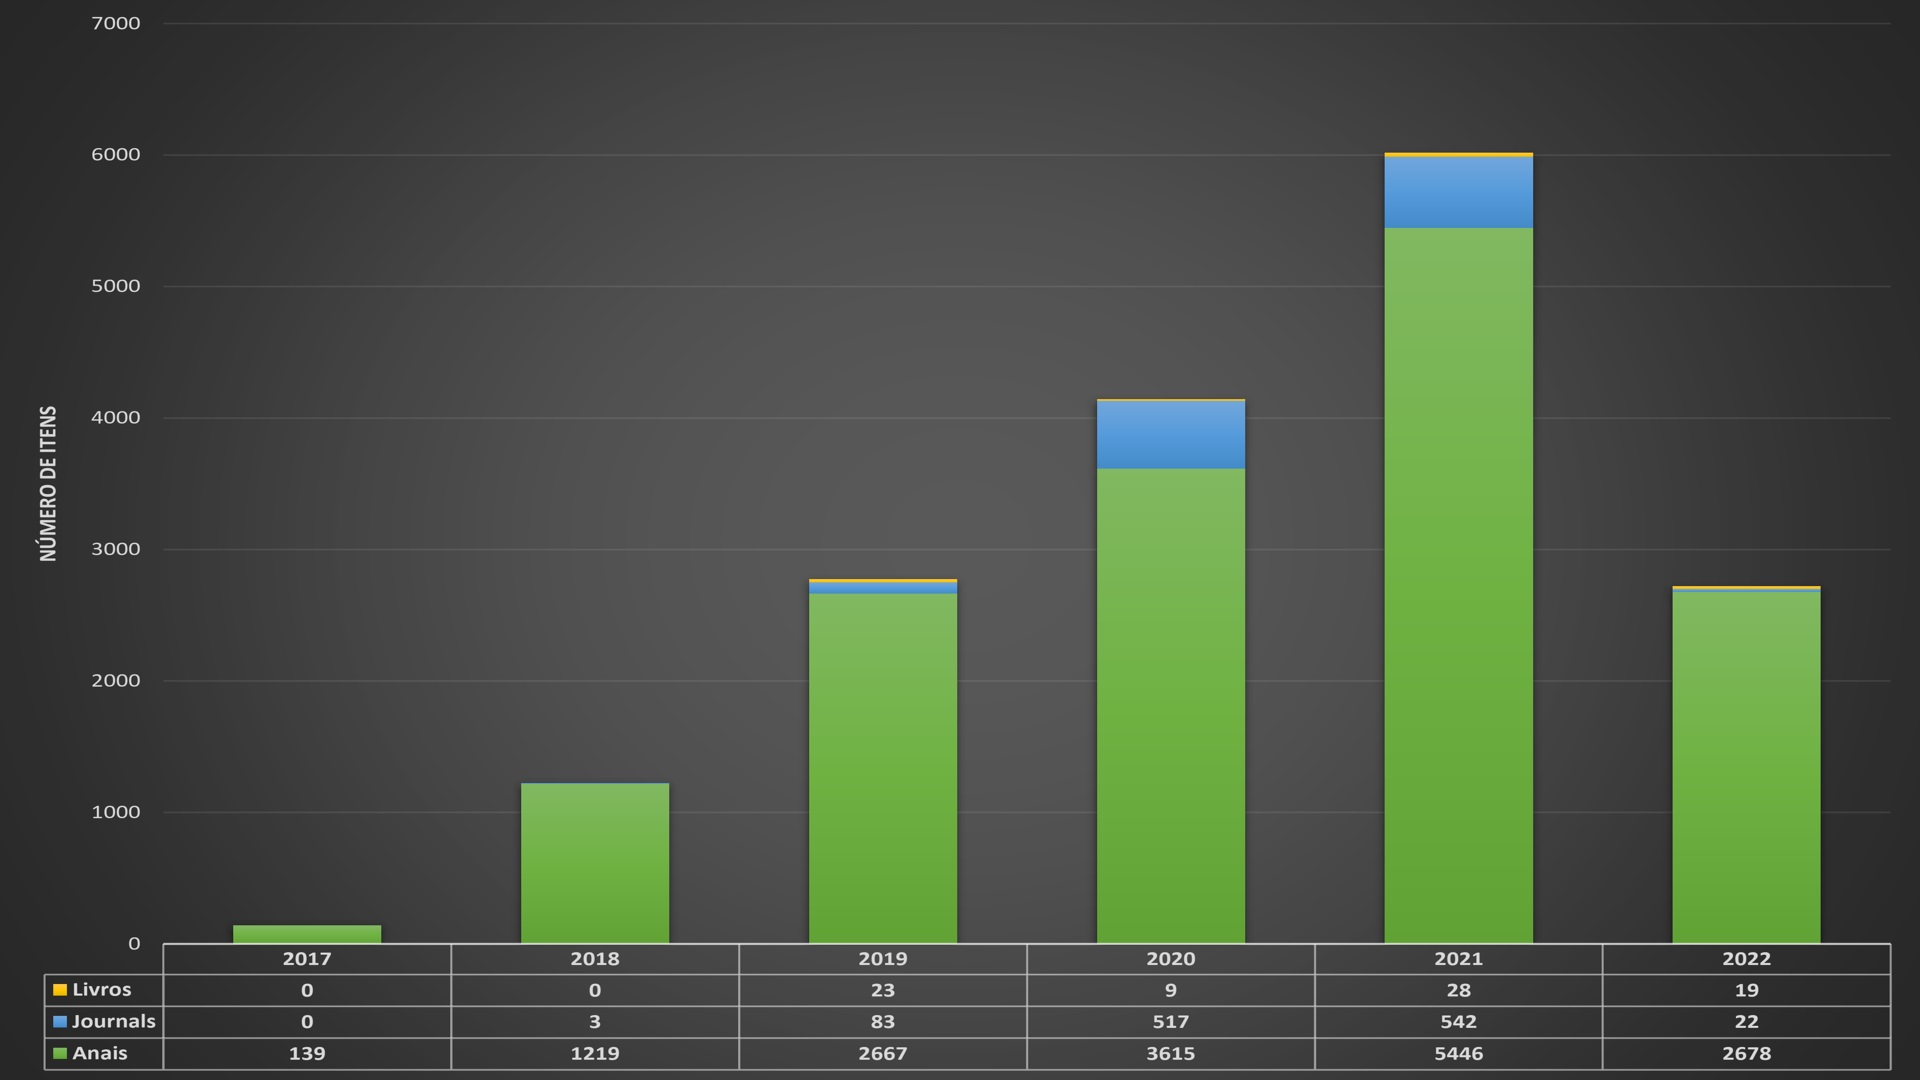
\includegraphics[width=30pc]{imagens/sol.jpg}
\caption{{Exemplo de legenda de figura.}}
 \label{Fig2}
\end{center}
\end{figure*}



\subsection{Exemplos com tabelas nativas}

\begin{table}[!ht]
\caption{Exemplo de legenda de tabela.}
\centering
\begin{tabular}{@{}cc@{}}
\hline\hline
Dimensão & Classificação\\
\hline%
 1  & 0.6232 \\
 2  & 0.9635 \\ 
 3  & 0.9724 \\ 
 4  & 0.9690 \\ 
 5  & 0.9840 \\ 
 6  & 0.9842 \\ 
 7  & 0.9873 \\ 
 8  & 0.9884 \\
 9  & 0.9873 \\ 
 10 & 0.9898 \\ 
 11 & 0.9914 \\
\hline\hline
\end{tabular}
\label{tab1}
\end{table}

Este é um texto para exemplificar como citar tabelas no decorrer do texto (ver \textbf{ Tabela~\ref{tab1}}). Como neste exemplo, é comum as tabelas aparecerem no arquivo \textit{.pdf} em um lugar distinto do que foram escritas no arquivo \texttt{.tex}. 

\subsection{Exemplo de tabelas com o pacote \texttt{tabularray}.  }


\begin{table}[!ht]
\caption{Exemplo de legenda de tabela.}
\centering
\begin{tblr}{%
columns={c},
row{even}={gray9},
row{1}={bg=gray!70, font=\bfseries}
}
\hline
Dimensão & Classificação\\
\hline%
 1  & 0.6 \\
 2  & 0.963 \\ 
 3  & 0.97 \\ 
 4  & 0.9690 \\ 
 5  & 0.9840 \\ 
 6  & 0.98423 \\ 
 7  & 0.9873 \\ 
 8  & 0.9884 \\
 9  & 0.9873 \\ 
 10 & 0.9898 \\ 
 11 & 0.991 \\
\end{tblr}
\label{tab1-1}
\end{table}


\subsection{Exemplos de citação dentro do texto}
Exemplo de citação de uma referencia (com o nome do autor antes do ano) \cite{ref3}. Outro exemplo, agora com autor e anos juntos \citep{ref4}. E mais um exemplo para a lista de referências ficar grande \citep{ref2,ref3,ref4}


\subsubsection{Equações}
\paragraph{Exemplo de Título Nível 4 (Parágrafo).}
Aqui temos um exemplo de equação no texto. Seja
\[
x=(x_1,\dots,x_n)\in R^n
\] ser um vetor \(n\)-dimensional. Aqui temos uma equação com \textit{label} para referências cruzadas.
\begin{equation}\label{eq1}
\max\limits_{x}\{x^TAx-\rho\|x\|_0:x^Tx=1\},
\end{equation}
E um exemplo de citação da Equação (\ref{eq1}). 

\paragraph{Outro Exemplo de Título Nível 4.} \lipsum[1]

\subsection{Exemplo de citação longa}
\begin{quotation}
\textit{Esta é uma citação longa. Lorem ipsum dolor sit amet, consectetur adipiscing elit, sed do eiusmod tempor incididunt ut labore et dolore magna aliqua. Lorem ipsum dolor sit amet, consectetur adipiscing elit, sed do eiusmod tempor incididunt ut labore et magna aliqua \citep{ref5}.
}\end{quotation} 



\subsection{Exemplo de tabela em duas colunas}

A Tabela \ref{tab2} é uma tabela que se expande tomando as duas colunas do documento. 

\begin{table*}
\caption{Exemplo de legenda de tabela pegando as duas colunas..} 
\centering
\begin{tabular*}{\textwidth}{@{}c\x c\x c\x c\x c\x c\x c\x c\x c\x c\x c\x c@{}}
\hline \hline
 Número   &  Vel (km/h)   & $\alpha$ (m/s$^2$)    &  $\epsilon^{(1)}$  &  $\epsilon^{(2)}$ 
         & $\delta^{(1)}$ & $\delta^{(2)}$  &  $\delta^{(3)}$    & $\gamma^{(1)}$ 
         & $\gamma^{(2)}$ & $\alpha^{(1)}$  & $\alpha^{(2)}$ \\
%
\hline
 1 & 3.5 & 2.0 & 0.20 & -0.05 & 0.00 & -0.20 & -0.05 & 0.20 & ~0.05 & 20 & 10 \\ 
 2 & 2.5 & 1.5 & 0.10 & -0.15 & 0.05 & -0.15 & ~0.00 & 0.10 & -0.05 & 20 & 40 \\ 
 3 & 3.0 & 1.8 & 0.20 & -0.05 & 0.25 & ~0.05 & ~0.20 & 0.15 & ~0.00 & 20 & 70$^a$ \\
\hline \hline
\end{tabular*}\label{tab2}
\end{table*}


 \section{Resultados (esperados)}
\label{sec:resultados}

Um parágrafo para preencher a seção. {\color{blue}\lipsum[1]}
 \section{Conclusão}
\label{sec:conclusao}

Um parágrafo para preencher a seção. {\color{blue}\lipsum[1]}

% ============
\begin{declarations}

\begin{acknowledgements}
ESTA DECLARAÇÃO É OPCIONAL. Este é um texto de agradecimentos com várias linhas. Lorem ipsum dolor sit amet, consectetur adipiscing elit, sed do eiusmod tempor incididunt ut labore et dolore magna aliqua. Ut enim ad minim veniam, quis nostrud exercitation ullamco laboris nisi ut aliquip ex ea commodo consequat.
\end{acknowledgements}

\begin{funding}
ESTA DECLARAÇÃO É OPCIONAL. Esta pesquisa foi financiada por lorem ipsum dolor sit amet, consectetur adipiscing elit.
\end{funding}

\begin{contributions}
ESTA DECLARAÇÃO É OBRIGATÓRIA. Sugerimos que os autores descrevam sua contribuição usando a Taxonomia CRediT (\href{https://credit.niso.org/}{https://credit.niso.org/}) como neste exemplo: JV contribuiu para a concepção deste estudo. CB, RP e CM realizaram os experimentos. JV é o principal contribuidor e escritor deste manuscrito. Todos os autores leram e aprovaram o manuscrito final. 
\end{contributions}

\begin{interests}
ESTA DECLARAÇÃO É OBRIGATÓRIA. Se não houver conflitos de interesse, os autores devem declarar: ``Os autores declaram que não têm nenhum conflito de interesses''. Caso contrário, a declaração deve ser: ``Os autores declaram que têm os seguintes conflito de interesses: lorem ipsum dolor sit amet, consectetur adipiscing elit.''
\end{interests}

\begin{materials}
ESTA DECLARAÇÃO É OBRIGATÓRIA. 
  Se os autores estiverem disponibilizando seus dados e/ou códigos
  abertamente, a declaração deve ser: ``Os conjuntos de dados (e/ou
  softwares) gerados e/ou analisados durante o estudo atual estão
  disponíveis em \ldots''. Caso contrário, a declaração deve ser: ``Os
  conjuntos de dados (e/ou softwares) gerados e/ou analisados durante
  o estudo atual serão feitos mediante solicitação''.
\end{materials}

\begin{furtherinformation}
ESTA DECLARAÇÃO É DESEJÁVEL. Informações adicionais relevantes, como, por exemplo, a aprovação em comitê de ética ou o uso de ferramentas de IA generativa no desenvolvimento do artigo. Essa declaração é opcional, se não houver nada a ser acrescentado, pode ser deixada em branco
\end{furtherinformation}
\end{declarations}



\bibliographystyle{apalike-sol}
\bibliography{referencias}
\appendix

\section{Um exemplo de Apêndice}

{\color{blue}\lipsum[1-5]}

\end{document}
